%\documentclass[hyperref={pdfpagelabels=false},slidetop,9pt]{beamer}
\documentclass[slidetop,8pt]{beamer}
\usepackage[T1]{fontenc}
\usepackage[utf8]{inputenc}
\newcommand{\id}{71}
\newcommand{\nom}{Théorie des mécanismes}
\newcommand{\sequence}{04}
\newcommand{\nomsequence}{Liaisons entre les solides}
\newcommand{\num}{02}
\newcommand{\type}{KH}
\newcommand{\descrip}{Liaisons équivalentes, hyperstatisme, liaisons en série et en parallèle, théorie des graphes}
\newcommand{\competences}{B2-12: Proposer une modélisation des liaisons avec leurs caractéristiques géométriques. \\ &  B2-13: Proposer un modèle cinématique paramétré à partir d'un système réel, d'une maquette numérique ou d'u \\ &  B2-17: Simplifier un modèle de mécanisme. \\ &  B2-18: Modifier un modèle pour le rendre isostatique. \\ &  C1-04: Proposer une démarche permettant d'obtenir une loi entrée-sortie géométrique.  \\ &  C2-05: Caractériser le mouvement d'un repère par rapport à un autre repère. \\ &  C2-06: Déterminer les relations entre les grandeurs géométriques ou cinématiques. }
\newcommand{\nbcomp}{7}
\newcommand{\systemes}{}
\newcommand{\systemesnum}{}
\newcommand{\systemessansaccent}{}
\newcommand{\ilot}{2}
\newcommand{\ilotstr}{02}
\newcommand{\dossierilot}{\detokenize{Ilot_02 }}

\usepackage{etex}
\usepackage{tikz}
\usepackage[european]{circuitikz}
\usepackage{pgf}
\usepackage[all]{xy}
\usepackage{pgfpages}
\usepackage{graphbox}
\usepackage{pdfpages}
%\usepackage[adobe-utopia]{mathdesign}
\usepackage{ifthen}
\usepackage{cancel}
\usepackage{framed}
\usepackage{subfig}
\usepackage{tabularx}
\usepackage{setspace}
\usepackage{soul}
\usepackage{schemabloc}
\usepackage{eqnarray}
\usepackage[dot, phantomtext]{dashundergaps}
\usepackage{media9}
\usepackage{multimedia}
\usepackage{textcomp}
\usefonttheme[onlymath]{serif}

\author{Renaud Costadoat}
\institute{Lycée Dorian}

\usepackage{multido}
\usepackage{multirow}
\usepackage{multicol} % Portions de texte en colonnes
\usepackage{flafter}%floatants après la référence

\usepackage{color}
\usepackage{xcolor}
\usepackage{colortbl}

\usepackage[gen]{eurosym}
\usepackage{tikz}
%\usepackage{pstricks,pst-node,pst-tree,pst-solides3d}
\usepackage{lmodern}
\usepackage[francais]{babel}
\usepackage{pslatex}
\usetheme{renaud}
\usepackage{times}
\usepackage[frenchmath]{newtxsf} % for sans serif symbols
\renewcommand{\familydefault}{\sfdefault}
%\usepackage{amsfonts}
%\usepackage{amsmath}
%\usepackage{mathastext}
\usepackage{verbatim}
\usepackage{moreverb}
%\usetikzlibrary{arrows,shapes}
\usepackage{graphicx}
\usepackage{psfrag}
\usepackage{wrapfig}
\usepackage{etoolbox}

\definecolor{gris25}{gray}{0.75}
\definecolor{bleu}{RGB}{18,33,98}
\definecolor{bleuf}{RGB}{42,94,171}
\definecolor{bleuc}{RGB}{231,239,247}
\definecolor{rougef}{RGB}{185,18,27}
\definecolor{rougec}{RGB}{255,188,204}%255,230,231
\definecolor{vertf}{RGB}{103,126,82}
\definecolor{vertc}{RGB}{220,255,191}

\setlength\parindent{24pt}
\parskip 7.2pt
\parindent 8pt

\newenvironment{rem}[1][\hsize]%
{%
    \def\FrameCommand
   {%
\rotatebox{90}{\textit{\textsf{Remarque}}} 
       {\color{bleuf}\vrule width 3pt}%
       \hspace{0pt}%must no space.
       \fboxsep=\FrameSep\colorbox{bleuc}%
  }%
    \MakeFramed{\hsize#1\advance\hsize-\width\FrameRestore}%
}%
{\endMakeFramed}%


\newenvironment{savoir}[1][\hsize]%
{%
    \def\FrameCommand
    {%
\rotatebox{90}{\textit{\textsf{Savoir}}} 
        {\color{bleuf}\vrule width 3pt}%
        \hspace{0pt}%must no space.
        \fboxsep=\FrameSep\colorbox{bleuc}%
    }%
    \MakeFramed{\hsize#1\advance\hsize-\width\FrameRestore}%
}%
{\endMakeFramed}%

\newenvironment{prob}[1][\hsize]%
{%
    \def\FrameCommand%
    {%
\rotatebox{90}{\textit{\textsf{Problematique}}} 
        {\color{rougef}\vrule width 3pt}%
        \hspace{0pt}%must no space.
        \fboxsep=\FrameSep\colorbox{rougec}%
    }%
    \MakeFramed{\hsize#1\advance\hsize-\width\FrameRestore}%
}%
{\endMakeFramed}%

\newenvironment{obj}[1][\hsize]%
{%
    \def\FrameCommand%
    {%
\rotatebox{90}{\textit{\textsf{Objectif}}} 
        {\color{vertf}\vrule width 3pt}%
        \hspace{0pt}%must no space.
        \fboxsep=\FrameSep\colorbox{vertc}%
    }%
    \MakeFramed{\hsize#1\advance\hsize-\width\FrameRestore}%
}%
{\endMakeFramed}%

\newenvironment{defi}[1][\hsize]%
{%
    \def\FrameCommand%
    {%
\rotatebox{90}{\textit{\textsf{Definition}}} 
        {\color{bleuf}\vrule width 3pt}%
        \hspace{0pt}%must no space.
        \fboxsep=\FrameSep\colorbox{rougec}%
    }%
    \MakeFramed{\hsize#1\advance\hsize-\width\FrameRestore}%
}%
{\endMakeFramed}%


\newenvironment{hypo}[1][\hsize]%
{%
    \def\FrameCommand%
    {%
\rotatebox{90}{\textit{\textsf{Hypothèse\\}}} 
        {\color{bleuf}\vrule width 3pt}%
        \hspace{0pt}%must no space.
        \fboxsep=\FrameSep\colorbox{bleuc}%
    }%
    \MakeFramed{\hsize#1\advance\hsize-\width\FrameRestore}%
}%
{\endMakeFramed}%


\newenvironment{prop}[1][\hsize]%
{%
    \def\FrameCommand%
    {%
\rotatebox{90}{\textit{\textsf{Propriété}}} 
        {\color{bleuf}\vrule width 3pt}%
        \hspace{0pt}%must no space.
        \fboxsep=\FrameSep\colorbox{bleuc}%
    }%
    \MakeFramed{\hsize#1\advance\hsize-\width\FrameRestore}%
}%
{\endMakeFramed}%

\newenvironment{props}[1][\hsize]%
{%
    \def\FrameCommand%
    {%
\rotatebox{90}{\textit{\textsf{Propriétés}}} 
        {\color{bleuf}\vrule width 3pt}%
        \hspace{0pt}%must no space.
        \fboxsep=\FrameSep\colorbox{bleuc}%
    }%
    \MakeFramed{\hsize#1\advance\hsize-\width\FrameRestore}%
}%
{\endMakeFramed}%

\newenvironment{exemple}[1][\hsize]%
{%
    \def\FrameCommand%
    {%
\rotatebox{90}{\textit{\textsf{Exemple}}} 
        {\color{vertf}\vrule width 3pt}%
        \hspace{0pt}%must no space.
        \fboxsep=\FrameSep\colorbox{vertc}%
    }%
    \MakeFramed{\hsize#1\advance\hsize-\width\FrameRestore}%
}%
{\endMakeFramed}%

\newenvironment{resultat}[1][\hsize]%
{%
    \def\FrameCommand%
    {%
\rotatebox{90}{\textit{\textsf{Résultat}}} 
        {\color{rougef}\vrule width 3pt}%
%        {\color{bleuf}\vrule width 3pt}%
        \hspace{0pt}%must no space.
        \fboxsep=\FrameSep\colorbox{rougec}%
    }%
    \MakeFramed{\hsize#1\advance\hsize-\width\FrameRestore}%
}%
{\endMakeFramed}%

\newenvironment{methode}[1][\hsize]%
{%
    \def\FrameCommand%
    {%
\rotatebox{90}{\textit{\textsf{Méthode\\}}} 
        {\color{rougef}\vrule width 3pt}%
        \hspace{0pt}%must no space.
        \fboxsep=\FrameSep\colorbox{rougec}%
    }%
    \MakeFramed{\hsize#1\advance\hsize-\width\FrameRestore}%
}%
{\endMakeFramed}%

\newenvironment{theo}[1][\hsize]%
{%
    \def\FrameCommand%
    {%
\rotatebox{90}{\textit{\textsf{Théorème\\}}} 
        {\color{rougef}\vrule width 3pt}%
        \hspace{0pt}%must no space.
        \fboxsep=\FrameSep\colorbox{rougec}%
    }%
    \MakeFramed{\hsize#1\advance\hsize-\width\FrameRestore}%
}%
{\endMakeFramed}%

\newenvironment{warn}[1][\hsize]%
{%
    \def\FrameCommand%
    {%
\rotatebox{90}{\textit{\textsf{Attention\\}}} 
        {\color{rougef}\vrule width 3pt}%
        \hspace{0pt}%must no space.
        \fboxsep=\FrameSep\colorbox{rougec}%
    }%
    \MakeFramed{\hsize#1\advance\hsize-\width\FrameRestore}%
}%
{\endMakeFramed}%

% \usepackage{pstricks}
%\usepackage{minitoc}
% \setcounter{minitocdepth}{4}

\setcounter{tocdepth}{2}

% \mtcselectlanguage{french} 

%\usepackage{draftcopy}% "Brouillon"
% \usepackage{floatflt}
\usepackage{psfrag}
%\usepackage{listings} % Permet d'insérer du code de programmation
\renewcommand{\baselinestretch}{1.2}

% Changer la num�rotation des figures :
% ------------------------------------
% \makeatletter
% \renewcommand{\thefigure}{\ifnum \c@section>\z@ \thesection.\fi
%  \@arabic\c@figure}
% \@addtoreset{figure}{section}
% \makeatother
 


%%%%%%%%%%%%
% Définition des vecteurs %
%%%%%%%%%%%%
 \newcommand{\vect}[1]{\overrightarrow{#1}}

%%%%%%%%%%%%
% Définition des torseusr %
%%%%%%%%%%%%

 \newcommand{\torseur}[1]{%
\left\{{#1}\right\}
}

\newcommand{\torseurcin}[3]{%
\left\{\mathcal{#1} \left(#2/#3 \right) \right\}
}

\newcommand{\torseurstat}[3]{%
\left\{\mathcal{#1} \left(#2\rightarrow #3 \right) \right\}
}

 \newcommand{\torseurc}[8]{%
%\left\{#1 \right\}=
\left\{
{#1}
\right\}
 = 
\left\{%
\begin{array}{cc}%
{#2} & {#5}\\%
{#3} & {#6}\\%
{#4} & {#7}\\%
\end{array}%
\right\}_{#8}%
}

 \newcommand{\torseurcol}[7]{
\left\{%
\begin{array}{cc}%
{#1} & {#4}\\%
{#2} & {#5}\\%
{#3} & {#6}\\%
\end{array}%
\right\}_{#7}%
}

 \newcommand{\torseurl}[3]{%
%\left\{\mathcal{#1}\right\}_{#2}=%
\left\{%
\begin{array}{l}%
{#1} \\%
{#2} %
\end{array}%
\right\}_{#3}%
}

 \newcommand{\vectv}[3]{%
\vect{V\left( {#1} \in {#2}/{#3}\right)}
}


\newcommand{\vectf}[2]{%
\vect{R\left( {#1} \rightarrow {#2}\right)}
}

\newcommand{\vectm}[3]{%
\vect{\mathcal{M}\left( {#1}, {#2} \rightarrow {#3}\right)}
}


 \newcommand{\vectg}[3]{%
\vect{\Gamma \left( {#1} \in {#2}/{#3}\right)}
}

 \newcommand{\vecto}[2]{%
\vect{\Omega\left( {#1}/{#2}\right)}
}

\newcommand{\reponse}[1][4]
{
\multido{}{#1}
{
\begin{center}
\makebox[0.9\linewidth]{\dotfill} \end{center}
}}


% }$$\left\{\mathcal{#1} \right\}_{#2} =%
% \left\{%
% \begin{array}{c}%
%  #3 \\%
%  #4 %
% \end{array}%
% \right\}_{#5}}


%  ------------------------------------------
% | Modification du formatage des sections : | 
%  ------------------------------------------

% Grands titres :
% ---------------

\newcommand{\titre}[1]{%
\begin{center}
      \bigskip
      \rule{\textwidth}{1pt}
      \par\vspace{0.1cm}
      
      \textbf{\large #1}
      \par\rule{\textwidth}{1pt}
    \end{center}
    \bigskip
  }

% Supprime le numéro du chapitre dans la numérotation des sections:
% -----------------------------------------------------------------
\makeatletter
\renewcommand{\thesection}{\@arabic\c@section}
\makeatother


% \titleformat{\chapter}[display]
% {\normalfont\Large\filcenter}
% {}
% {1pc}
% {\titlerule[1pt]
%   \vspace{1pc}%
%   \Huge}[\vspace{1ex}%
% \titlerule]


%%%% Chapitres Comme PY Pechard %%%%%%%%%
% numéro du chapitre
\DeclareFixedFont{\chapnumfont}{OT1}{phv}{b}{n}{80pt}
% pour le mot " Chapitre "
\DeclareFixedFont{\chapchapfont}{OT1}{phv}{m}{it}{40pt}
% pour le titre
\DeclareFixedFont{\chaptitfont}{T1}{phv}{b}{n}{25pt}

\definecolor{gris}{gray}{0.75}
\setbeamertemplate{section in toc}[sections numbered]

\newlength{\RoundedBoxWidth}
\newsavebox{\GrayRoundedBox}
\newenvironment{GrayBox}[1][\dimexpr\textwidth-4.5ex]%
   {\setlength{\RoundedBoxWidth}{\dimexpr#1}
    \begin{lrbox}{\GrayRoundedBox}
       \begin{minipage}{\RoundedBoxWidth}}%
   {   \end{minipage}
    \end{lrbox}
    \begin{center}
    \begin{tikzpicture}%
       \draw node[draw=bleuf,fill=bleuc,rounded corners,%
             inner sep=2ex,text width=\RoundedBoxWidth]%
             {\usebox{\GrayRoundedBox}};
    \end{tikzpicture}
    \end{center}}
    
\ifdef{\prive}{\pgfpagesuselayout{2 on 1}[a4paper,border shrink=0mm]}
\ifdef{\prive}{\setbeamertemplate{navigation symbols}{}}
\setbeamertemplate{itemize item}[ball]
%\setbeamertemplate{blocks}[rounded]%[shadow=true]
\setbeamercolor{block title}{fg=white,bg=grisf}        % titre block normal 
\setbeamercolor{block body}{fg=grisf,bg=grisc!50}      % corps block normal
\setbeamercolor{block body alerted}{fg=white,bg=warning}   % idem pour un block alerte

\title{\nom}
\date{S\sequence \ - \type\num}

\begin{document}
\shorthandoff{:!}
\bibliographystyle{abbrvnat-fr}

\usebackgroundtemplate%
{%
    \centering
\includegraphics[width=\paperwidth]{/home/renaud/Documents/Renaud/GitHub/Sciences-Ingenieur/img/fond2}%
}

{
\setbeamertemplate{navigation symbols}{}
\setbeamertemplate{headline}[pagetitre]
\setbeamertemplate{footline}[pagetitre]
\usebackgroundtemplate{\centering
\includegraphics[width=\paperwidth]{/home/renaud/Documents/Renaud/GitHub/Sciences-Ingenieur/img/fond}}
\frame{\titlepage}
}



\section{Dipôles électriques}

\setcounter{framenumber}{0}

{\frame{
\frametitle{Introduction}

\begin{savoir}
Vous êtes capables :
\begin{itemize}
 \item de modéliser la chaîne d'énergie d'un système,
 \item d'en concevoir une partie.
\end{itemize}
\end{savoir}

\begin{prob}
Vous devez êtes capables :
\begin{itemize}
 \item d'analyser et de modéliser un circuit électrique,
 \item de modéliser les sources électriques,
 \item de manipuler les lois de l'électrocinétique.
\end{itemize}
\end{prob}
}}

{\frame{
\frametitle{L'électronique}

Les lois de \textbf{l'électronique} que nous allons étudier seront valables dans le cadre de:
\begin{itemize}
 \item l'électronique du signal,
 
 \begin{minipage}{0.35\linewidth}
  \begin{itemize}
   \item Capteur, potentiomètre,...
   \item Filtre,...
   \item Lampe, Haut parleur,...
  \end{itemize}
 \end{minipage}\hfill
  \begin{minipage}{0.6\linewidth}
  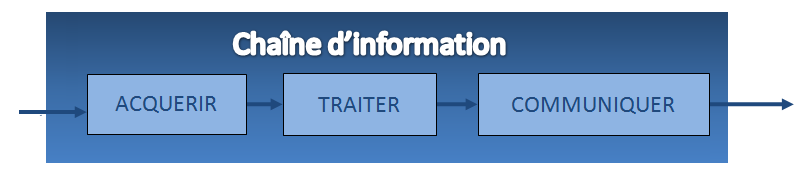
\includegraphics[width=0.9\linewidth]{img/Chaine_info}
 \end{minipage}

\vfill

 \item l'électronique de puissance (chaîne d'énergie).

 \begin{minipage}{0.35\linewidth}
  \begin{itemize}
   \item Transformateur, redresseur,
   \item Variateur, hacheur, onduleur,...
  \end{itemize}
 \end{minipage}\hfill
  \begin{minipage}{0.6\linewidth}
  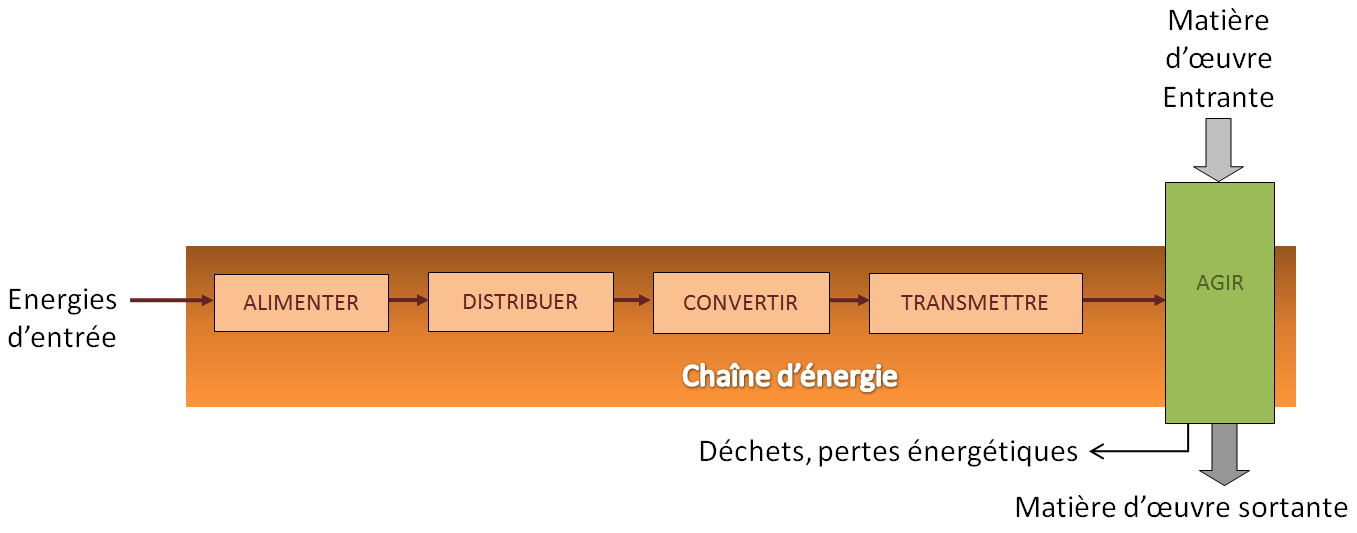
\includegraphics[width=0.9\linewidth]{img/Chaine_energie}
 \end{minipage}
\end{itemize}
}}

{\frame{
\frametitle{Électronique du signal}

L'électronique du signal correspond à l'étude de l'acquisition, du traitement et de la communication d'un signal électrique de faible puissance ($\leq 1 Watt$).

\hfill

\begin{minipage}{0.3\linewidth}
\begin{flushleft}
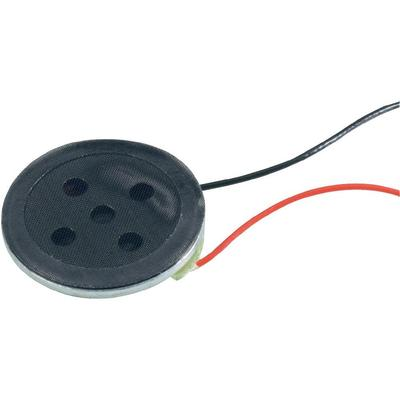
\includegraphics[width=2cm]{img/HP}
\end{flushleft}
\end{minipage}
\hfill
\begin{minipage}{0.3\linewidth}
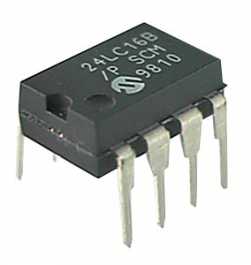
\includegraphics[width=1.5cm]{img/aop}
\end{minipage}
\hfill
\begin{minipage}{0.3\linewidth}
\begin{flushright}
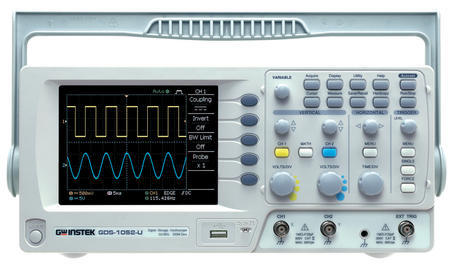
\includegraphics[width=3cm]{img/oscillo}
\end{flushright}
\end{minipage}

\hfill

\begin{rem}
\begin{minipage}{0.7\linewidth}
Cette partie de l'électronique sera étudiée en Physique.
\begin{itemize}
 \item Signal, Circuits, Filtres,...
\end{itemize}
\end{minipage} \hfill
\begin{minipage}{0.25\linewidth}
\begin{flushright}
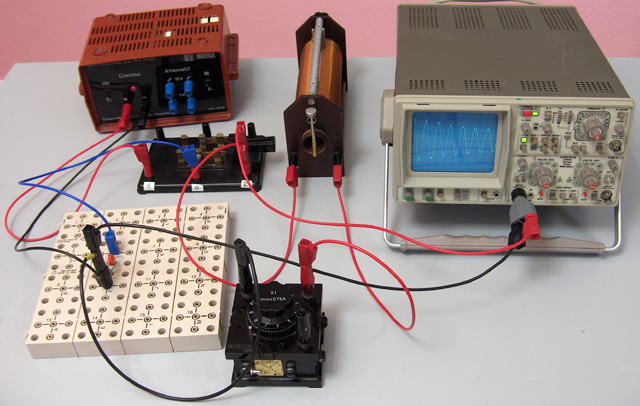
\includegraphics[width=2cm]{img/montage_phys}
\end{flushright}
\end{minipage}
\end{rem}
}}

{\frame{
\frametitle{Électronique de puissance}

\textbf{L'électronique de puissance} est une branche de l'électrotechnique qui concerne les dispositifs permettant de changer la forme de l'énergie électrique (convertisseurs).

Aujourd'hui près de 15\% de l'énergie électrique produite est convertie sous une forme ou une autre. 

\begin{center}
\begin{tabular}{|c|c|}
\hline
Lampe éco (onduleur) & Drone (hacheur+onduleur)  \\
 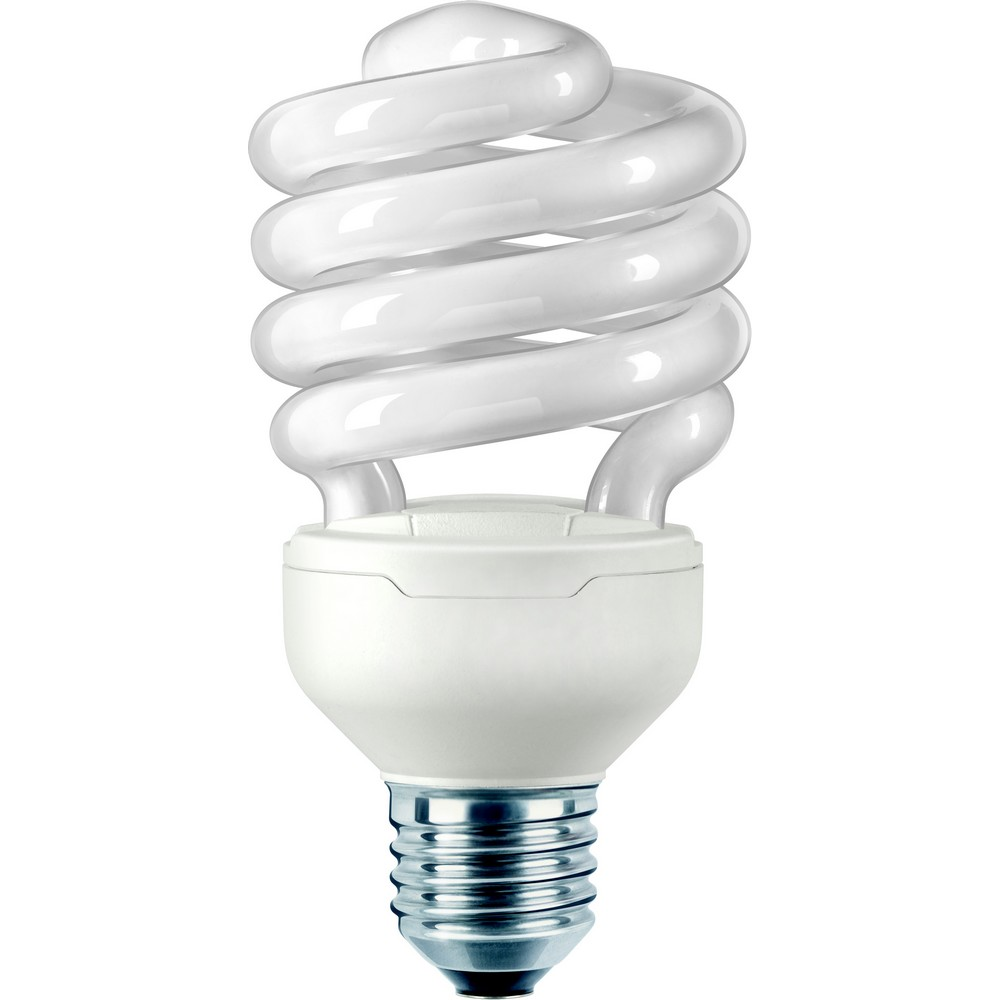
\includegraphics[height=2cm]{img/lampe} &  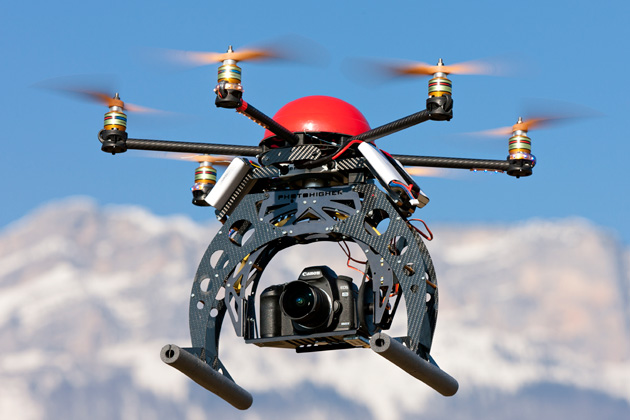
\includegraphics[height=2cm]{img/drone} \\
\hline
\multicolumn{2}{|c|}{Panneau solaire et onduleur} \\
\multicolumn{2}{|c|}{ 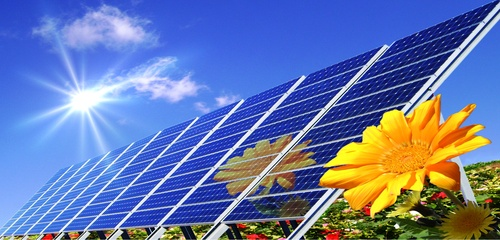
\includegraphics[height=1.5cm]{img/panneau_photo} \hfill
 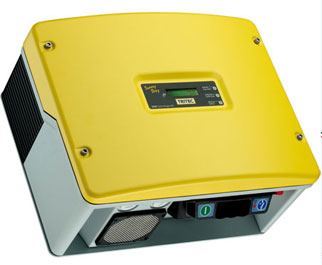
\includegraphics[height=1.5cm]{img/onduleur}} \\
 \hline
\end{tabular}
\end{center}
}}

{\frame{
\frametitle{Électronique de commutation}

L'objectif de l'électronique de \textbf{commutation} est d'\textbf{adapter} et de \textbf{distribuer} une énergie électrique pour son utilisation tout en garantissant des rendements très importants.

Pour cela, elle s'appuie sur des principes de \textbf{commutation}. En effet, idéalement, un interrupteur ouvert ou fermé ne dissipe pas d'énergie Ainsi, il est possible en théorie d'effectuer un \textbf{transfert contrôlé} d'énergie entre une \textbf{source d'entrée} et une \textbf{charge de sortie}.

\tikzstyle{int}=[draw, fill=blue!20, minimum size=2em]
\tikzstyle{init} = [pin edge={to-,thin,black}]

\begin{figure}[!h]
\begin{center}
\begin{tikzpicture}[node distance=2.5cm,auto,>=]%latex']
    \node [int, text width=1.7cm, align=center] (a) {ALIMENTER: Source};
    \node [int, right of=a, node distance=3cm, text width=1.7cm, align=center] (b) {DISTRIBUER:  Cellule de commutation};
    \node [int, right of=b, node distance=3cm, text width=1.7cm, align=center] (c) {CONVERTIR:  Charge};
    \path[->] (a) edge node {} (b);
    \draw[->] (b) edge node {} (c);
\end{tikzpicture}
\end{center}
\caption{Intégration d'une cellule de commutation dans la chaîne d'énergie}
\end{figure}

\begin{itemize}
 \item \textbf{Source:} \textbf{continue} (batterie, ...) ou \textbf{alternative} (réseau, ...).
 \item \textbf{Charge:} \textbf{courant continu} (moteur CC, résistance,...) ou \textbf{courant alternatif} (moteur synchrone, asynchrone,...).
\end{itemize}

L'étude des cellules de commutation fera l'objet d'un cours particulier.
}}



{\frame{
\frametitle{Dipôles}

La majorité des composants en électroniques possèdent deux bornes, il sont alors appelés \og dipôles \fg.

\begin{defi}
Un \textbf{dipôle} est un système accessible par deux \textbf{bornes} dans lequel peut circuler un \textbf{courant électrique}.
\end{defi}

\begin{itemize}
 \item Pour qu'un courant puisse circuler dans un dipôle, il faut brancher celui-ci sur un autre dipôle.
 \item Un dipôles peut être actif ou passif.
\end{itemize}

Le comportement électrique d'un dipôle est caractérisé par deux grandeurs: 
\begin{itemize}
 \item la tension (force): différence de potentiel aux bornes du dipôle (en Volt $V$),
 \item le courant (flux): intensité du courant traversant le dipôle (en Ampère $A$).
\end{itemize}
}}

{\frame{
\frametitle{Types de dipôles}

\textbf{Dipôle passif}

Si on branche ensemble deux dipôles identiques et qu'aucun courant permanent ne passe entre les
deux dipôles quel que soit le sens du branchement, ces dipôles sont passifs.

\begin{small}
	\begin{itemize}
 		\item Il va circuler du courant dans un dipôle passif si on applique une différence de potentiel entre ses
bornes,
		\item Réciproquement, si on fait circuler un courant dans ce dipôle, il va apparaître une tension à ses
bornes,
		\item \textit{Exemples: résistances, thermistances, condensateurs}
	\end{itemize}
\end{small}

~\

\textbf{Dipôle actif}

Si on branche un dipôle sur une résistance et qu'un courant permanent circule, alors ce dipôle est
actif.

\begin{small}
	\begin{itemize}
		\item \textit{Exemples: pile, accumulateur, alternateur},
		\item \textit{Remarque:} Bien qu'ils ne répondent pas intrinsèquement à la définition ci-dessus, on classera également dans cette catégorie les semi-conducteurs et circuits intégrés ayant des caractéristiques de générateurs :
diodes, zéners, transistors.
	\end{itemize}
\end{small}

}}

{\frame{
\frametitle{Principaux dipôles passifs idéaux}

\begin{itemize}
 \item Les \textbf{résistances pures}:

\begin{minipage}{0.7\linewidth}
Relation instantanée courant/tension: \textbf{$u(t)=R.i(t)$}

\begin{itemize}
 \item $R$ constant quelles que soient les conditions d'utilisation,
 \item Impédance complexe en régime sinusoïdal : $R$.
\end{itemize}

\end{minipage}
\hfill
\begin{minipage}{0.25\linewidth}
 \centering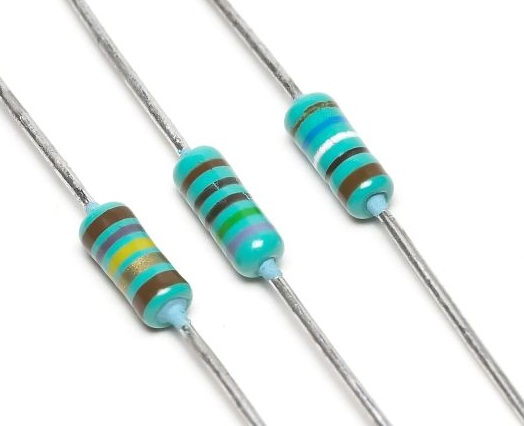
\includegraphics[height=1.5cm]{img/resistors}
\end{minipage}

\vfill

 \item Les \textbf{inductances pures}:

\begin{minipage}{0.7\linewidth}
Relation instantanée courant/tension: \textbf{$u(t)=L\cdot\frac{di(t)}{dt}$}

\begin{itemize}
 \item $L$ constant quelles que soient les conditions d'utilisation,
 \item Impédance complexe en régime sinusoïdal : $j.L\omega$,
 \item Énergie emmagasinée par la bobine : $W_L=\frac{1}{2}.L.i^2$
\end{itemize}

\end{minipage}
\hfill
\begin{minipage}{0.25\linewidth}
 \centering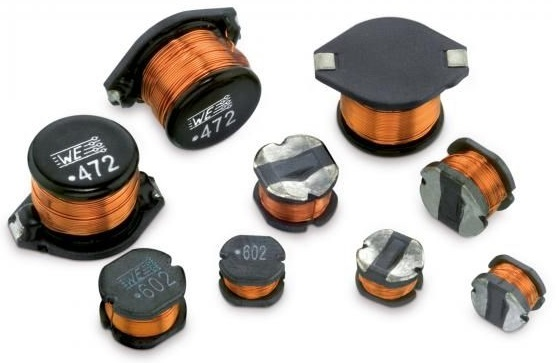
\includegraphics[height=1.5cm]{img/bobines}
\end{minipage}

\vfill

 \item Les \textbf{condensateurs parfaits}:

\begin{minipage}{0.7\linewidth}
Relation instantanée courant/tension: \textbf{$i(t)=C\cdot\frac{du(t)}{dt}$}

\begin{itemize}
 \item $C$ constant quelles que soient les conditions d'utilisation,
 \item Impédance complexe en régime sinusoïdal : $1/j.C\omega$,
 \item Énergie emmagasinée par le condensateur : $W_C=\frac{1}{2}.C.u^2$
\end{itemize}
\end{minipage}
\hfill
\begin{minipage}{0.25\linewidth}
 \centering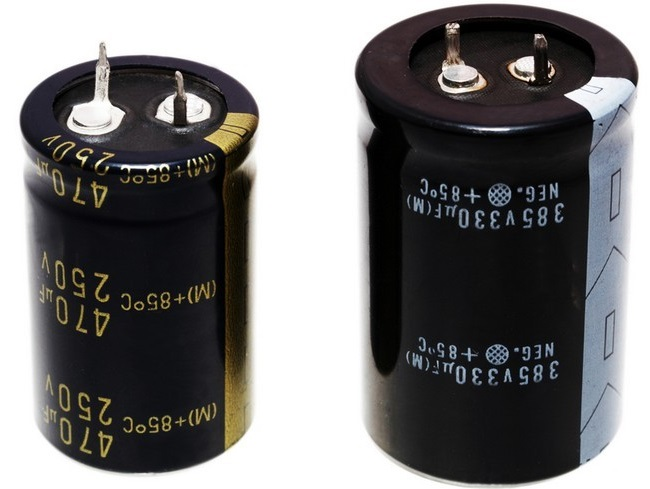
\includegraphics[height=1.3cm]{img/condensateur}
\end{minipage}
\end{itemize}
}}


\section{Sources électriques}

{\frame{
\frametitle{Sources (dipôle actifs) parfaites}

\begin{minipage}{0.7\linewidth}

\textbf{Source de tension}

Un dipôle est une source de tension s'il maintient la \textbf{même tension} entre ses bornes, et ce quel que soit le courant qu'il débite ou qu'il absorbe.

\begin{small}
	\begin{itemize}
 		\item Une source de tension est un dipôle actif,
 		\item Elle est \textbf{continue} si la tension est fixe dans le temps,
 		\item Elle est \textbf{alternative} si la tension varie dans le temps de façon périodique.
	\end{itemize}
\end{small}
\end{minipage}\hfill
\begin{minipage}{0.25\linewidth}
\begin{center}
\begin{circuitikz}
\ctikzset{bipoles/length=0.8cm}
\draw[color=bleuf] (0,1.5) to[V, v=$u$, l_=Source continue] (0,2.5);
\draw[color=bleuf] (0,0) to[sV, v=$u$, l_=Source alternative] (0,1);
\end{circuitikz}
\end{center}
\end{minipage}

\vfill

\begin{minipage}{0.7\linewidth}

\textbf{Sources de courant}

Un dipôle est une source de courant s'il débite le \textbf{même courant}, et ce quelle que soit la tension entre ses bornes.

\begin{small}
	\begin{itemize}
 		\item Une source de courant est un dipôle actif,
 		\item Elle est \textbf{continue} si le courant est fixe dans le temps,
 		\item Elle est \textbf{alternative} si le courant varie dans le temps de façon périodique.
	\end{itemize}
\end{small}
\end{minipage}\hfill
\begin{minipage}{0.25\linewidth}
\begin{circuitikz}
\ctikzset{bipoles/length=0.8cm}
\draw[color=bleuf] (0,1.5) to[I, i=$i$, l_=Source continue] (0,2.5);
\draw[color=bleuf] (0,0) to[sI, i=$i$, l_=Source alternative] (0,1);
\end{circuitikz}
\end{minipage}
}}

{\frame{
\frametitle{Sources réelles}

Les modèles précédents sont des modèles théoriques, en réalité:
\begin{itemize}
  \item Une source de tension aura une impédance série non nulle (\textit{Modèle de Thévenin}),
  \item Une source de courant aura une impédance parallèle non nulle (\textit{Modèle de Norton}).
\end{itemize}
\begin{center}
 \begin{circuitikz}[scale=0.8]
\ctikzset{bipoles/length=0.8cm}
\draw[color=bleuf] (2,0) -- (0,0) to[V, v=$u$] (0,2) to[R, l^=$R$] (2,2) ;
\draw[color=bleuf] (5,0) -- (3,0) to[I, i=$i$] (3,2) -- (5,2) ;
\draw[color=bleuf] (4,0) to[R, l^=$R$] (4,2) ;
\draw (2.5,0) node[below] {Sources de tension et de courant réelles};
\end{circuitikz}
\end{center}

\begin{defi}
L'impédance électrique mesure l'opposition d'un circuit électrique au passage d'un courant alternatif sinusoïdal. La définition d'impédance est une généralisation de la loi d'Ohm dans l'étude des circuits en courant alternatif.
\end{defi}
}}

{\frame{
\frametitle{Conventions de signe}

\begin{minipage}{0.7\linewidth}

\textbf{Convention générateur}

\begin{small}
\begin{itemize}
 \item Un dipôle est \textbf{générateur} lorsqu'il \textbf{fournit de l'énergie} (même de manière très temporaire).
 \item Le courant \textbf{sort par le pôle positif} du dipôle générateur (flèches dans le même sens).
\end{itemize}
\end{small}
\end{minipage}\hfill
\begin{minipage}{0.25\linewidth}
 \begin{circuitikz}[scale=0.8]
\ctikzset{bipoles/length=0.8cm}
\draw[color=bleuf] (0,0) to[generic, l^=$\overrightarrow{\hspace{0.4cm}V\hspace{0.4cm}}$, i=$i$] (2,0) ;
\end{circuitikz}
\end{minipage}

\vfill

\begin{minipage}{0.7\linewidth}

\textbf{Convention récepteur}

\begin{small}
\begin{itemize}
 \item Un dipôle est un \textbf{récepteur} quand il \textbf{consomme de l'énergie}.
 \item Courant et tension sont orientés en sens inverse. Le pôle positif du dipôle est celui par lequel \textbf{rentre le courant}.
\end{itemize}
\end{small}
\end{minipage}\hfill
\begin{minipage}{0.25\linewidth}
 \begin{circuitikz}[scale=0.8]
\ctikzset{bipoles/length=0.8cm}
\draw[color=bleuf] (0,0) to[generic, l^=$\overleftarrow{\hspace{0.4cm}V\hspace{0.4cm}}$, i=$i$] (2,0) ;
\end{circuitikz}
\end{minipage}

\begin{rem}
 \begin{itemize}
  \item Attention à ne pas confondre \textbf{actif/générateur} et \textbf{passif/récepteur},
  \item Faire très attention au \textbf{sens des flèches} qui montre la différence entre les deux.
 \end{itemize}  
\end{rem}

}}


{\frame{
\frametitle{Association de dipôles}

Quand on connecte deux dipôles ensemble, ils présentent la même tension à leurs bornes (!), et le courant entrant dans l'un est égal au courant sortant de l'autre.

~\

\begin{minipage}{0.6\linewidth}

\textbf{Association passif / actif}

\begin{small}
La tension aux bornes des deux dipôles étant la même, il y en aura un avec le courant dans le même sens que la tension et l'autre avec le courant en sens inverse. L'un délivre de l'énergie que l'autre absorbe.
\end{small}
\end{minipage}\hfill
\begin{minipage}{0.35\linewidth}

\begin{center}
\begin{circuitikz}
\ctikzset{bipoles/length=0.8cm}
\draw[color=bleuf] (0,0) to[V, v=$u$, i>=$i$] (0,2) -- (2,2)
to [R, l=$R$] (2,0) -- (0,0);
\draw (1,2) node {$\bullet$} node [above left] {A};
\draw (1,0) node {$\bullet$} node [above left] {B};
\draw[-triangle 45] (1,0.2) -- (1,1.8) node[right, midway] {$V_{AB}$};
\end{circuitikz}
\end{center}
\end{minipage}

\begin{minipage}{0.6\linewidth}

\textbf{Association actif / actif}

\begin{small}
Le courant ainsi orienté sortira par le pôle positif du dipôle générateur. L'autre dipôle actif est utilisé en récepteur (courant entrant par le pôle positif). L'association de sources fera l'objet d'une étude plus détaillée.
\end{small}
\end{minipage}\hfill
\begin{minipage}{0.35\linewidth}
\begin{center}
\begin{circuitikz}
\ctikzset{bipoles/length=0.8cm}
\draw[color=bleuf] (0,0) to[V, v=$u_1$, i>=$i$] (0,1) to[R, l=$R_1$] (0,2)
 -- (2,2) to[R, l=$R_2$] (2,1) to[V, v<=$u_2$,i>_=$i$] (2,0) -- (0,0) ;
\draw (1,2) node {$\bullet$} node [above left] {A};
\draw (1,0) node {$\bullet$} node [above left] {B};
\draw[-triangle 45] (1,0.2) -- (1,1.8) node[right, midway] {$V_{AB}$};
\end{circuitikz}
\end{center}
\end{minipage}
}}


{\frame{
\frametitle{Association de sources}

L'association de dipôles actifs peut être effectuée mais il faut être prudent car certaines configurations sont impossible à cause de la nature des sources. C'est le cas des quatre suivantes.

\vfill

\textbf{Sources de tension}

\vfill

\begin{minipage}{0.6\linewidth}
\begin{small}
Il ne faut jamais \textbf{disposer deux sources de tension en parallèle}. Cela reviendrait à imposer deux tensions différentes entre deux mêmes points d'un circuit.
\end{small}
\end{minipage}\hfill
\begin{minipage}{0.35\linewidth}

\begin{center}
\begin{circuitikz}
 \ctikzset{bipoles/length=0.8cm}
 \draw[color=bleuf] (0,0) to[V, v=$u_1$] (0,1) -- (1,1)
 to[V, v<=$u_2$] (1,0) -- (0,0);
 \draw[color=rougef](-0.5,-0.5) -- (1.5,1.5);
 \draw[color=rougef](-0.5,1.5) -- (1.5,-0.5);
\end{circuitikz}
\end{center}
\end{minipage}

\vfill

\begin{minipage}{0.6\linewidth}
\begin{small}
Il ne faut jamais \textbf{court-circuiter une source de tension}. Cela entraînerai la circulation d'un courant infini.
\end{small}
\end{minipage}\hfill
\begin{minipage}{0.35\linewidth}

\begin{center}
\begin{circuitikz}
 \ctikzset{bipoles/length=0.8cm}
 \draw[color=bleuf] (0,0) to[V, v=$u_1$] (0,1) -- (1,1) -- (1,0) -- (0,0);
 \draw[color=rougef](-0.5,-0.5) -- (1.5,1.5);
 \draw[color=rougef](-0.5,1.5) -- (1.5,-0.5);
\end{circuitikz}
\end{center}
\end{minipage}
}}

{\frame{
\frametitle{Association de sources}

L'association de dipôles actifs peut être effectuée mais il faut être prudent car certaines configurations sont impossible à cause de la nature des sources. C'est le cas des quatre suivantes.

\textbf{Sources de courant}

\begin{minipage}{0.6\linewidth}
\begin{small}
Il ne faut jamais \textbf{disposer deux sources de courant en série}. Cela reviendrait à imposer deux courants différents dans la même branche.
\end{small}
\end{minipage}\hfill
\begin{minipage}{0.35\linewidth}

\begin{center}
\begin{circuitikz}
 \ctikzset{bipoles/length=0.8cm}
 \draw[color=bleuf] (0,0) to[I, i=$i_1$] (0,1) to[I, i=$i_2$] (0,2);
 \draw[color=rougef](-0.5,-0.25) -- (0.5,2.25);
 \draw[color=rougef](0.5,-0.25) -- (-0.5,2.25);
\end{circuitikz}
\end{center}
\end{minipage}

\begin{minipage}{0.6\linewidth}
\begin{small}
Il ne faut jamais \textbf{ouvrir} un circuit dans lequel se trouve une \textbf{source de courant}. Cela entraînerai une tension infinie à ses bornes.
\end{small}
\end{minipage}\hfill
\begin{minipage}{0.35\linewidth}

\begin{center}
\begin{circuitikz}
 \ctikzset{bipoles/length=0.8cm}
 \draw[color=bleuf] (1,0) -- (0,0) to[I, i=$i_1$] (0,1) -- (1,1);
 \draw[color=rougef](-0.5,-0.25) -- (1.5,1.25);
 \draw[color=rougef](-0.5,1.25) -- (1.5,-0.25);
\end{circuitikz}
\end{center}
\end{minipage}
}}

\section{Les lois de l'électrocinétique} 

{\frame{
\frametitle{Les lois de l'électrocinétique}

\begin{defi}
\textbf{L'électrocinétique} correspond à l'étude des circuits électriques. Celle-ci s'effectue en supposant les régimes \textbf{quasi stationnaires}.
\end{defi}

\vfill

Ainsi, en supposant les régimes quasi stationnaires l'électricité est considérée comme un fluide parfait et incompressible. L'intensité du courant qui entre à l'extrémité d'un conducteur est alors exactement identique à celle qui sort à l'autre extrémité.

\vfill

Il est alors possible d'étudier :
\begin{itemize}
 \item La typologie des circuits,
 \item Les dipôles,
 \item Le comportement des circuits lorsqu'ils sont soumis à des tensions particulières.
\end{itemize}

}}

{\frame{
\frametitle{Les lois de Kirchhoff}

Les deux principales lois de l'électrocinétiques sont les deux lois de Krichhoff:
\begin{itemize}
 \item la loi des mailles,
 \item la loi des n\oe uds.
\end{itemize}

Le circuit suivant sera utilisé à titre d'exemple.

\begin{center}
\begin{circuitikz}
\ctikzset{bipoles/length=0.8cm}
\draw[color=bleuf] (2,0) -- (0,0) to[V, i>=$i_1$] (0,1) to[R, l_=$R_1$] (0,2) -- (2,2);
\draw[color=bleuf] (2,2) -- (4,2) to [R, l_=$R_2$] (4,1) to[V, i<^=$i_2$] (4,0) -- (2,0);
\draw[color=bleuf] (2,2) to[R, i=$i_3$, l_=$R_3$] (2,0);
\draw (2,2) node {$\bullet$} node [above left] {A};
\draw (2,0) node {$\bullet$} node [above left] {B};
\draw[-triangle 45] (-0.4,0.2) -- (-0.4,0.8) node[left, midway] {$V_{1}$};
\draw[triangle 45-] (-0.4,1.2) -- (-0.4,1.8) node[left, midway] {$U_{R1}$};
\draw[-triangle 45] (2.3,0.2) -- (2.3,1.8) node[right, midway] {$U_{R3}$};
\draw[-triangle 45] (4.4,0.2) -- (4.4,0.8) node[right, midway] {$V_{2}$};
\draw[triangle 45-] (4.4,1.2) -- (4.4,1.8) node[right, midway] {$U_{R2}$};
\end{circuitikz}
\end{center}

}}

{\frame{
\frametitle{La loi des mailles}


\begin{defi}
La loi des mailles définit une relation vectorielle entre les tensions. En parcourant une maille dans un sens de rotation choisi arbitrairement, toutes les tensions fléchée dans le même sens de rotation sont additionnées, les autres sont soustraites.
\end{defi}

\begin{minipage}{0.45\linewidth}
Maille 1 \\
\begin{circuitikz}
\ctikzset{bipoles/length=0.8cm}
\draw[color=bleuf] (2,0) -- (0,0) to[V, i>=$i_1$] (0,1) to[R, l_=$R_1$] (0,2) -- (2,2);
\draw[color=bleuf, dashed] (2,2) -- (4,2) to [R, l_=$R_2$] (4,1) to[V, i<^=$i_2$] (4,0) -- (2,0);
\draw[color=bleuf] (2,2) to[R, i=$i_3$, l_=$R_3$] (2,0);
\draw (2,2) node {$\bullet$} node [above left] {A};
\draw (2,0) node {$\bullet$} node [above left] {B};
\draw[-triangle 45] (-0.4,0.2) -- (-0.4,0.8) node[left, midway] {$V_{1}$};
\draw[triangle 45-] (-0.4,1.2) -- (-0.4,1.8) node[left, midway] {$U_{R1}$};
\draw[-triangle 45] (2.3,0.2) -- (2.3,1.8) node[right, midway] {$U_{R3}$};
\end{circuitikz}
Ici, $V_1-U_{R1}-U_{R3}=0$.
\end{minipage}\hfill
\begin{minipage}{0.45\linewidth}
Maille 2 \\
\begin{circuitikz}
\ctikzset{bipoles/length=0.8cm}
\draw[color=bleuf, dashed] (2,0) -- (0,0) to[V, i>=$i_1$] (0,1) to[R, l_=$R_1$] (0,2) -- (2,2);
\draw[color=bleuf] (2,2) -- (4,2) to [R, l_=$R_2$] (4,1) to[V, i<^=$i_2$] (4,0) -- (2,0);
\draw[color=bleuf] (2,2) to[R, i=$i_3$, l_=$R_3$] (2,0);
\draw (2,2) node {$\bullet$} node [above left] {A};
\draw (2,0) node {$\bullet$} node [above left] {B};
\draw[-triangle 45] (2.3,0.2) -- (2.3,1.8) node[right, midway] {$U_{R3}$};
\draw[-triangle 45] (4.4,0.2) -- (4.4,0.8) node[right, midway] {$V_{2}$};
\draw[triangle 45-] (4.4,1.2) -- (4.4,1.8) node[right, midway] {$U_{R2}$};
\end{circuitikz}
Ici, $U_{R3}+U_{R2}-V_2=0$.
\end{minipage}

La troisième maille aurait permis de trouver: $V_1-U_{R1}+U_{R2}-V_2=0$
}}

{\frame{
\frametitle{La loi des n\oe uds}

\begin{defi}
La loi des n\oe uds définit une relation entre les courant qui transitent par un n\oe ud. Un n\oe ud correspondant à la connexion d'au moins 3 branches. Il est alors possible d'écrire que la somme des courants entrants est égale à la somme des courants sortants.
\end{defi}

\begin{center}
\begin{circuitikz}
\ctikzset{bipoles/length=0.8cm}
\draw[color=bleuf] (2,0) -- (0,0) to[V, i>=$i_1$] (0,1) to[R, l_=$R_1$] (0,2) -- (2,2);
\draw[color=bleuf] (2,2) -- (4,2) to [R, l_=$R_2$] (4,1) to[V, i<^=$i_2$] (4,0) -- (2,0);
\draw[color=bleuf] (2,2) to[R, i=$i_3$, l_=$R_3$] (2,0);
\draw (2,2) node {$\bullet$} node [above left] {A};
\draw (2,0) node {$\bullet$} node [above left] {B};
\draw[-triangle 45] (-0.4,0.2) -- (-0.4,0.8) node[left, midway] {$V_{1}$};
\draw[triangle 45-] (-0.4,1.2) -- (-0.4,1.8) node[left, midway] {$U_{R1}$};
\draw[-triangle 45] (2.3,0.2) -- (2.3,1.8) node[right, midway] {$U_{R3}$};
\draw[-triangle 45] (4.4,0.2) -- (4.4,0.8) node[right, midway] {$V_{2}$};
\draw[triangle 45-] (4.4,1.2) -- (4.4,1.8) node[right, midway] {$U_{R2}$};
\end{circuitikz}
\end{center}

Ici, $i_1+i_2=i_3$.

Cette modélisation nous permet alors de trouver les équations qui lient les courants et les tensions du circuit aux caractéristiques des dipôles.
}}

{\frame{
\frametitle{Mise en équation}

\begin{minipage}{0.2\linewidth}
\begin{circuitikz}
\ctikzset{bipoles/length=0.8cm}
\draw[color=bleuf] (0,0) to[R, l_=$R_1$, i=$i_1$] (0,1.5);
\draw[triangle 45-] (-0.4,0.2) -- (-0.4,1.3) node[left, midway] {$U_{R1}$};
\end{circuitikz}
\end{minipage}\hfill
\begin{minipage}{0.75\linewidth}
Les caractéristiques des résistances nous donnent: \\ $U_{R1}=R_1.i_1$, $U_{R2}=R_2.i_2$, $U_{R3}=R_3.i_3$. \\
Les équations de la loi des mailles deviennent alors:
$\left\{\begin{array}{l}
V_1-R_1.i_1-R_3.i_3=0 \\
R_3.i_3+R_2.i_2-V_2=0
\end{array}\right.$
\end{minipage}

\begin{minipage}{0.4\linewidth}
En ajoutant les résultats de la loi des n\oe uds:$i_1+i_2=i_3$.

$\left\{\begin{array}{l}
V_1-(R_1+R_3).i_1-R_3.i_2=0 \\
R_3.i_1+(R_2+R_3).i_2-V_2=0
\end{array}\right.$
\end{minipage}\hfill
\begin{minipage}{0.4\linewidth}
\begin{resultat}
$i_1=\dfrac{(R_2+R_3).V_1-R_3.V_2}{R_1.R_2+R_1.R_3+R_2.R_3}$
\end{resultat}
\end{minipage}


\begin{center}
\begin{circuitikz}
\ctikzset{bipoles/length=0.5cm}
\draw[color=bleuf] (2,0) -- (0,0) to[V, i>=$i_1$] (0,1) to[R, l_=$R_1$] (0,2) -- (2,2);
\draw[color=bleuf] (2,2) -- (4,2) to [R, l_=$R_2$] (4,1) to[V, i<^=$i_2$] (4,0) -- (2,0);
\draw[color=bleuf] (2,2) to[R, i=$i_3$, l_=$R_3$] (2,0);
\draw (2,2) node {$\bullet$} node [above left] {A};
\draw (2,0) node {$\bullet$} node [above left] {B};
\draw[-triangle 45] (-0.4,0.2) -- (-0.4,0.8) node[left, midway] {$V_{1}$};
\draw[triangle 45-] (-0.4,1.2) -- (-0.4,1.8) node[left, midway] {$U_{R1}$};
\draw[-triangle 45] (2.3,0.2) -- (2.3,1.8) node[right, midway] {$U_{R3}$};
\draw[-triangle 45] (4.4,0.2) -- (4.4,0.8) node[right, midway] {$V_{2}$};
\draw[triangle 45-] (4.4,1.2) -- (4.4,1.8) node[right, midway] {$U_{R2}$};
\end{circuitikz}
\end{center}

}}

{\frame{
\frametitle{Association de résistances}

Des lois précédentes découlent des propriétés qui permettent la simplification de circuits.

\textbf{Résistances en série} \fbox{$R_{eq}=\sum R_i$}

\begin{center}
\begin{circuitikz}
\ctikzset{bipoles/length=0.8cm}
\draw[color=bleuf] (0,0) to[R, l^=$R_1$] (1,0) to[R, l^=$R_2$] (2,0) (3,0) to[R, l^=$R_n$] (4,0);
\draw[triangle 45-triangle 45] (4.5,0) -- (5.5,0);
\draw[color=bleuf] (6,0) to[R, l^=$R_{eq}$] (7,0);
\draw[color=bleuf, dashed] (2,0) -- (3,0);
\end{circuitikz}
\end{center}

\textbf{Résistances en parallèle} \fbox{$R_{eq}=\dfrac{1}{\sum \frac{1}{R_i}}$}

\begin{center}
\begin{circuitikz}
\ctikzset{bipoles/length=0.8cm}
\draw[color=bleuf] (0,0) to[R, l^=$R_1$] (0,2) (1,0) to[R, l^=$R_2$] (1,2) (3,0) to[R, l^=$R_n$] (3,2);
\draw[triangle 45-triangle 45] (3.5,1) -- (4.5,1);
\draw[color=bleuf] (5.5,0) to[R, l^=$R_{eq}$] (5.5,2);
\draw[color=bleuf] (0,0) -- (1.5,0);
\draw[color=bleuf] (0,2) -- (1.5,2);
\draw[color=bleuf, dashed] (1.5,0) -- (2.5,0);
\draw[color=bleuf, dashed] (1.5,2) -- (2.5,2);
\draw[color=bleuf] (2.5,0) -- (3,0);
\draw[color=bleuf] (2.5,2) -- (3,2);
\end{circuitikz}
\end{center}
}}

{\frame{
\frametitle{Théorème de superposition}

\begin{defi}
Une tension (ou courant) est égale à la somme de ces tensions pour chaque source indépendante seule, les autres étant "passivées".
\end{defi}

\begin{minipage}{0.45\linewidth}
\begin{itemize}
 \item Source de \textbf{tension} "passivée": \textit{fil},
 \item Source de \textbf{courant} "passivée": \textit{enlevée}.
\end{itemize}
\centering\fbox{$i_1=i'_1+i''_1$}
\end{minipage}
\begin{minipage}{0.45\linewidth}
\begin{center}
\begin{circuitikz}
\ctikzset{bipoles/length=0.8cm}
\draw[color=bleuf] (2,0) -- (0,0) to[V] (0,1) to[R, l_=$R_1$] (0,2) to[short, i_=$i_1$] (2,2);
\draw[color=bleuf] (2,2) -- (4,2) to [R, l_=$R_2$] (4,1) to[V] (4,0) -- (2,0);
\draw[color=bleuf] (2,2) to[R, i=$i_3$, l_=$R_3$] (2,0);
\draw (2,2) node {$\bullet$} node [above left] {A};
\draw (2,0) node {$\bullet$} node [above left] {B};
\draw[-triangle 45] (-0.4,0.2) -- (-0.4,0.8) node[left, midway] {$V_{1}$};
\draw[-triangle 45] (4.4,0.2) -- (4.4,0.8) node[right, midway] {$V_{2}$};
\end{circuitikz}
\end{center}
\end{minipage}

\begin{minipage}{0.45\linewidth}
\begin{circuitikz}
\ctikzset{bipoles/length=0.8cm}
\draw[color=bleuf] (2,0) -- (0,0) to[V] (0,1) to[R, l_=$R_1$] (0,2) to[short, i_=$i'_1$] (2,2);
\draw[color=bleuf] (2,2) -- (4,2) to [R, l_=$R_2$] (4,1) -- (4,0) -- (2,0);
\draw[color=bleuf] (2,2) to[R, i=$i_3$, l_=$R_3$] (2,0);
\draw (2,2) node {$\bullet$} node [above left] {A};
\draw (2,0) node {$\bullet$} node [above left] {B};
\draw[-triangle 45] (-0.4,0.2) -- (-0.4,0.8) node[left, midway] {$V_{1}$};
\end{circuitikz}
\end{minipage}+
\begin{minipage}{0.45\linewidth}
\begin{circuitikz}
\ctikzset{bipoles/length=0.8cm}
\draw[color=bleuf] (2,0) -- (0,0) -- (0,1) to[R, l_=$R_1$] (0,2) to[short, i_=$i''_1$] (2,2);
\draw[color=bleuf] (2,2) -- (4,2) to [R, l_=$R_2$] (4,1) to[V] (4,0) -- (2,0);
\draw[color=bleuf] (2,2) to[R, i=$i_3$, l_=$R_3$] (2,0);
\draw (2,2) node {$\bullet$} node [above left] {A};
\draw (2,0) node {$\bullet$} node [above left] {B};
\draw[-triangle 45] (4.4,0.2) -- (4.4,0.8) node[right, midway] {$V_{2}$};
\end{circuitikz}
\end{minipage}
}}

{\frame{
\frametitle{Pont diviseur de tension}

\begin{defi}
Le pont diviseur de tension est un montage classique qui permet de \textbf{réduire} une tension.
\end{defi}

\hfill

\begin{minipage}{0.49\linewidth}
\begin{center}
\begin{circuitikz}
\ctikzset{bipoles/length=0.8cm}
\draw[color=bleuf] (4,0) -- (0,0) to[V] (0,2) -- (2,2) to [R, l_=$R_1$] (2,1) to [R, l_=$R_2$] (2,0) ;
\draw[color=bleuf] (2,1) to[short, i={$i \thickapprox 0$}] (4,1) ;
\draw (2,1) node {$\bullet$} node [left] { A};
\draw (2,0) node {$\bullet$} node [below] { B};
\draw[-triangle 45] (-0.4,0.2) -- (-0.4,1.8) node[left, midway] {$U_{e}$};
\draw[-triangle 45] (4.4,0.2) -- (4.4,0.8) node[right, midway] {$U_{s}$};
\end{circuitikz}
\end{center}
\end{minipage}\hfill
\begin{minipage}{0.3\linewidth}
\fbox{$U_s=\dfrac{R_2}{R_1+R_2}.U_e$}
\end{minipage}
 }}

{\frame{
\frametitle{Théorème de Millman}

\begin{rem}
Lorsque plusieurs sources de tension réelles sont associées en parallèle, il est possible de calculer la tension globale grâce à la relation de Millman. Une source réelle étant modélisée par un modèle de Thévenin.
\end{rem}

\hfill

\begin{minipage}{0.48\linewidth}
\begin{center}
\begin{circuitikz}
\ctikzset{bipoles/length=0.8cm}
\draw[color=bleuf] (0,0) to[V, v=$U_1$] (0,1) to[R, l^=$R_1$] (0,2);
\draw[color=bleuf] (1,0) to[V, v=$U_2$] (1,1) to[R, l^=$R_2$] (1,2);
\draw[color=bleuf] (3,0) to[V, v=$U_i$] (3,1) to[R, l^=$R_i$] (3,2);
\draw[color=bleuf] (5,0) to[V, v=$U_n$] (5,1) to[R, l^=$R_n$] (5,2);
\draw[color=bleuf] (0,0) -- (2,0);
\draw[color=bleuf, dashed] (2,0) -- (2.8,0);
\draw[color=bleuf] (2.8,0) -- (3.2,0);
\draw[color=bleuf, dashed] (3.2,0) -- (4,0);
\draw[color=bleuf] (4,0) -- (5,0);
\draw[color=bleuf] (0,2) -- (2,2);
\draw[color=bleuf, dashed] (2,2) -- (2.8,2);
\draw[color=bleuf] (2.8,2) -- (3.2,2);
\draw[color=bleuf, dashed] (3.2,2) -- (4,2);
\draw[color=bleuf] (4,2) -- (5,2);
\draw[-triangle 45] (2,0.2) -- (2,1.8) node[left, midway] {$U$};
\end{circuitikz}
\end{center}
\end{minipage}\hfill
\begin{minipage}{0.38\linewidth}
\fbox{$V=\dfrac{\dfrac{V_1}{R_1}+\dfrac{V_2}{R_2}+...+\dfrac{V_i}{R_i}+...+\dfrac{V_n}{R_n}}{\dfrac{1}{R_1}+\dfrac{1}{R_2}+...+\dfrac{1}{R_i}+...+\dfrac{1}{R_n}}$}
\end{minipage}

\hfill

\begin{center}
\fbox{$V=\dfrac{\sum\limits_{i = 1}^n\dfrac{V_i}{R_i}}{\sum\limits_{i = 1}^n\dfrac{1}{R_i}}$}
\end{center}

}}

{\frame{
\frametitle{Électronique et électrocinétique}

\begin{savoir}
Vous devez être capables :
\begin{itemize}
 \item de modéliser un dipôle en fonction de ses caractéristiques,
 \item de manipuler des sources de tension et de courant,
 \item de modéliser un circuit et de déterminer ces caractéristiques grâce aux lois de l'électrocinétique.
\end{itemize}
\end{savoir}

\begin{prob}

Il est nécessaire d'utiliser d'autres formes de représentation d'un mécanisme.
\begin{itemize}
 \item \textit{Problème: Comment modéliser un convertisseur statique ?}
 \item \textbf{Perspectives}: Déterminer une méthode de modélisation et des critères de choix afin d'intégrer un convertisseur statique dans une chaîne d'énergie.
\end{itemize}
\end{prob}

}}

\end{document}